% !TeX root = skripta-konstitutivni-vztahy-materialu.tex
% !TeX lastmodified = 2019-12-04

\subsection{Model plastického zpevnění Voce4}\label{sec:model-voce-4}
Tento model je jedním z řady modelů testovaných autorem na různých slitinách a~vykazuje nejlepší shodu s~experimenty pro řadu materiálů s~výraznou mezí kluzu.
V~souřadnicích skutečné napětí vs. logaritmické přetvoření je dán rovnicí:
\begin{equation}
	\sigma = \sigma_y + C_1 \left[ 1 - \exp\left(-k_1 \varepsilon\right) \right] + C_2 \left[ 1 - \exp\left(-k_2 \varepsilon\right) \right]
\end{equation}
kde
\begin{description}
	\item[$\sigma_y$]je mez kluzu,
	\item[$\varepsilon$] je redukované plastické přetvoření
	\item[{$C_1, C_2  [MPa], k_1, k_2 [-]$}] jsou další parametry modelu.
\end{description}

\subsubsection{Porovnání modelu Voce4 s~experimenty}
\begin{figure}[H]
	\centering
	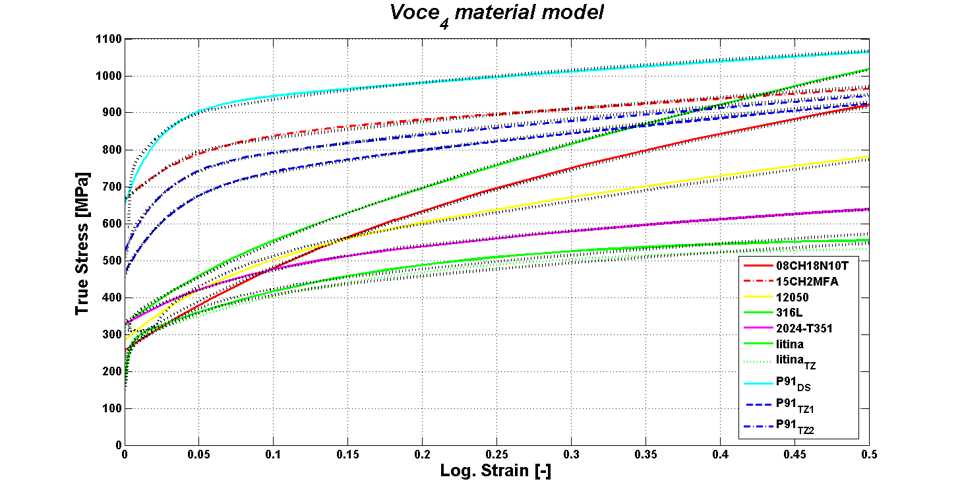
\includegraphics[width=0.9\linewidth]{aproximace-voce4}
	\caption{Porovnání modelu Voce4 s~experimenty (výsledky experimentů tečkovaně)}
	\label{fig:aproximace-voce4}
\end{figure}

\begin{itemize}
	\item Austenitické oceli\\
	\texttt{08CH18N10T} (ruská vysokolegovaná ocel používaná na jaderných zařízeních)\\
	\texttt{15CH2MFA} (ruská vysokolegovaná ocel používaná na jaderných zařízeních)\\
	\texttt{AISI 316L} (americká vysokolegovaná ocel používaná na energetických zařízeních)
	\item Feritické oceli\\
	\texttt{ČSN 41 2050} -- konstrukční uhlíková ocel vhodná pro zušlechťování a~kalení\\
	\texttt{P91} -- \texttt{X10CrMoVNb91} -- žárupevná, korozně odolná vůči páře, zplodinám hoření a~H2, v~základním a~dvou tepelně zpracovaných stavech.
	\item Tvárná litina \texttt{EN-GJS-400-18U-LT} -- s kuličkovým grafitem, která se používá na komponenty větrných elektráren a~její tažnost je min. $A = \SI{18}{\%}$, v~základním stavu a~tepelně zpracovaná.
	\item Dural \texttt{2024-T351} -- je slitina hliníku Al-Cu-Mg, hojně využívaná v~letectví, je charakteristická svou vysokou pevností.
\end{itemize}
